\section{Analisis Hasil Pengujian}

\subsection{Siklus Penjualan Tiket}

Kedua skenario pengujian ini memiliki siklus permintaan yang berbeda. Siklus dalam hal ini berarti fase ketika sistem memiliki pola permintaan yang berbeda. Contoh pada skenario beban berkelanjutan diambil dari pengujian f1t2, sedangkan contoh pada skenario perebutan tiket diambil dari pengujian f1t4. Siklus/pola ini juga terjadi pada skenario serupa ketika proses penjualan berjalan dengan lancar.

\subsubsection{Skenario Beban Berkelanjutan}

\begin{figure}[htbp]
    \centering
    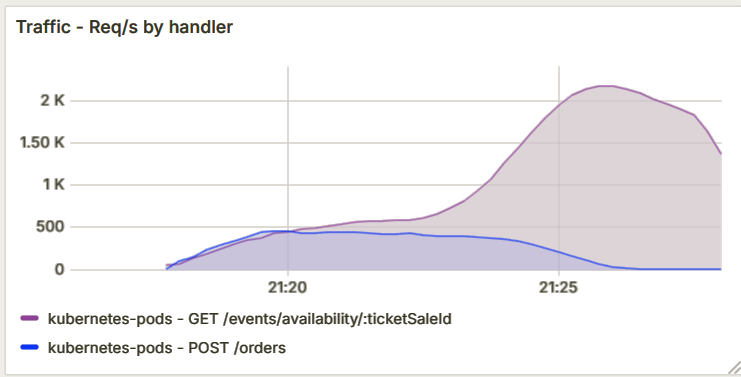
\includegraphics[width=0.6\textwidth]{resources/chapter-4/pattern-stress-traffic.png}
    \caption{Pola Permintaan pada Beban Berkelanjutan}
    \label{fig:pattern-stress-traffic}
\end{figure}

Pada skenario ini, sistem memiliki ketersediaan tiket yang banyak sehingga penjualan tiket yang berhasil berjalan cukup lama. Setelah tiket habis terjual, jumlah permintaan ketersediaan tiket jauh meningkat karena penguji mencoba mencari tiket dari berbagai area dengan lebih banyak.

\begin{figure}[htbp]
    \centering
    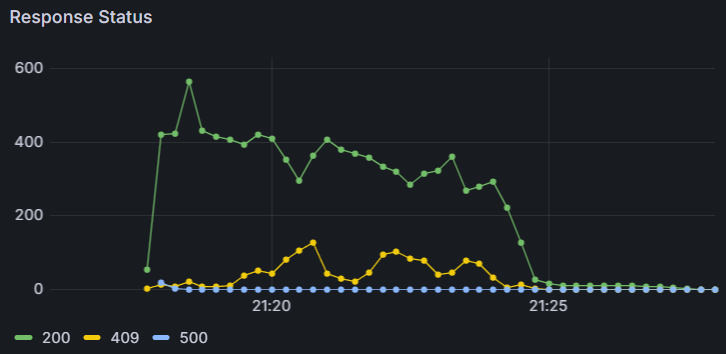
\includegraphics[width=0.6\textwidth]{resources/chapter-4/pattern-stress-order.png}
    \caption{Status Respons pada Beban Berkelanjutan}
    \label{fig:pattern-stress-order}
\end{figure}


Status respons pemesanan tiket menunjukkan bahwa terjadi konflik (kode 409) selama pemrosesan pesanan sebanyak 3-10\% dari respons secara keseluruhan.

\pagebreak

\subsubsection{Skenario Perebutan Tiket}

\begin{figure}[htbp]
    \centering
    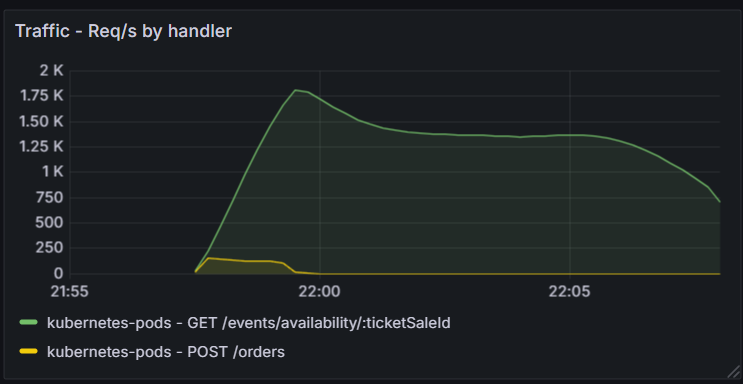
\includegraphics[width=0.6\textwidth]{resources/chapter-4/pattern-sim-traffic.png}
    \caption{Pola Permintaan pada Perebutan Tiket}
    \label{fig:pattern-sim-traffic}
\end{figure}

Pada skenario ini, jumlah permintaan ketersediaan jauh lebih banyak dibandingkan permintaan pemesanan tiket. Hal ini wajar karena terdapat lebih banyak peminat dibandingkan dengan tiket yang tersedia. Berdasarkan grafik di atas, tiket habis terjual dalam kurang lebih 2 menit penjualan.

\begin{figure}[htbp]
    \centering
    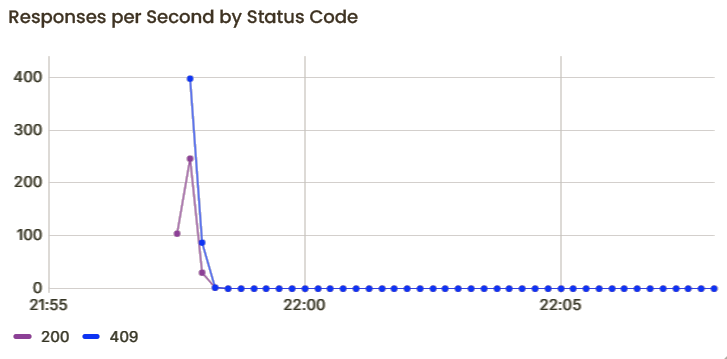
\includegraphics[width=0.6\textwidth]{resources/chapter-4/pattern-sim-order.png}
    \caption{Status Respons pada Perebutan Tiket}
    \label{fig:pattern-sim-order}
\end{figure}

Status respons pemesanan tiket menunjukkan bahwa terjadi konflik (kode 409) yang cukup banyak bahkan sejak proses penjualan dimulai. Pengguna yang baru masuk setelahnya pada akhirnya akan gagal memperoleh tiket, sebagaimana digambarkan pada keadaan akhir penguji pada gambar berikut.

\begin{figure}[htbp]
    \centering
    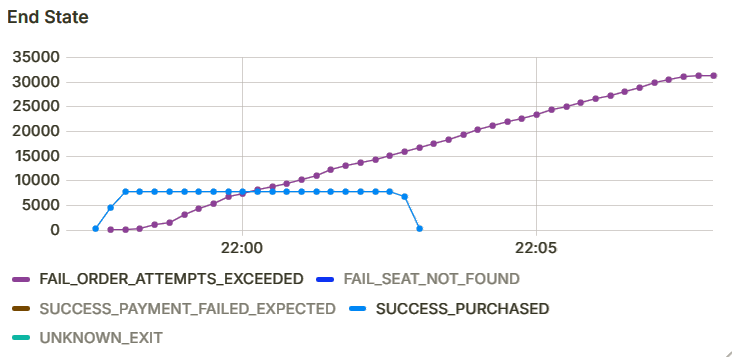
\includegraphics[width=0.6\textwidth]{resources/chapter-4/pattern-sim-k6.png}
    \caption{Keadaan Akhir Penguji pada Perebutan Tiket}
    \label{fig:pattern-sim-k6}
\end{figure}


\subsection{Kinerja Selama Pengujian}

Secara garis besar, varian PostgreSQL mampu menangani beban yang diberikan dengan sangat baik. Varian CitusData masih memiliki kinerja yang baik, meski memiliki latensi yang lebih tinggi dibandingkan dengan PostgreSQL. YugabyteDB mengalami lebih banyak kegagalan dan kinerja yang buruk sehingga tidak dapat menyelesaikan proses penjualan dengan baik. Sampel pengujian yang dipilih pada adalah skenario stress-2 tanpa pengendalian aliran. Skenario ini merupakan skenario pengujian dengan kinerja YugabyteDB yang dapat diterima dan mampu menyelesaikan proses penjualan. Dengan beban yang lebih tinggi, YugabyteDB mengalami banyak kegagalan. Pembahasan lebih lanjut hasil pelaksanaan setiap pengujian dibahas pada lampiran \ref{apx:test-run-performance}.

\begin{table}[h]
    \centering
    \caption{Gambaran Kinerja Permosesan Pesanan}
    \label{table:kinerja-pemrosesan-pesanan}
    \begin{tabular}{|l|l|l|l|}
        \hline
        \textbf{Metrik}              & \textbf{PostgreSQL} & \textbf{CitusData} & \textbf{YugabyteDB} \\
        \hline
        \textit{Throughput} Maksimum & 466 rps             & 410 rps            & 216 rps             \\
        \hline
        Penggunaan CPU (Puncak)      & 8 vCPU              & 10 vCPU            & 19 vCPU             \\
        \hline
        Penggunaan Memori (Puncak)   & 3.4 GB              & 5 GB               & 36 GB               \\
        \hline
        Latensi Pemrosesan (P50)     & 192-382 ms          & 496-650 ms         & 854-10000 ms        \\
        \hline
    \end{tabular}
\end{table}

Latensi dan \textit{throughput} pemrosesan diukur dari sisi Ticket Server, bukan dari level basis data. Latensi pemrosesan yang diambil merupakan latensi terbaik saat beban sudah cukup tinggi dan laju pemrosesan mulai stabil. Penggunaan CPU dan penggunaan memori merupakan agregat puncak jumlah penggunaan sumber daya setiap instans basis data yang berkaitan. Apabila terdapat dua nilai maksimal \textit{throughput} yang mendekati, nilai yang dipilih adalah nilai yang memiliki rasio sukses (kode respons 200) paling tinggi.

Berdasarkan tabel di atas, PostgreSQL unggul dari segala aspek, mulai dari laju pemrosesan, penggunaan sumber daya, serta latensi. CitusData memiliki laju pemrosesan yang mendekati PostgreSQL dengan latensi 2x lebih lambat dan penggunaan sumber daya yang sedikit lebih tinggi. Di sisi lain, YugabyteDB memiliki laju pemrosesan kurang dari setengah PostgreSQL dengan latensi setidaknya 4x lebih lambat, penggunaan CPU 2.4x lebih banyak, dan penggunaan memori 10x lebih banyak.

\subsection{Kinerja Basis Data Terdistribusi}

Sebagaimana digambarkan pada tabel \ref{table:kinerja-pemrosesan-pesanan}, kinerja PostgreSQL lebih baik dibandingkan CitusData dan YugabyteDB. Mari telusuri lebih dalam kinerja setiap basis data, terutama pada skenario lain.

\subsubsection{Rata-Rata Waktu Eksekusi Kueri}

Berikut adalah data rata-rata waktu eksekusi kueri yang diambil dari tabel pg\_stat\_statements sesaat setelah pengujian dilaksanakan. Data PostgreSQL diambil dari pengujian f1t2, CitusData diambil dari pengujian f2t3, dan YugabyteDB diambil dari f3t1. Beban antara PostgreSQL dan CitusData sama karena pengujian dijalankan pada skenario stress-0, sedangkan beban pada YugabyteDB lebih ringan karena dijalankan pada skenario stress-2. Data PostgreSQL merupakan gabungan antara statistik pada instans \textit{primary} dan replika. Data mentah merupakan data 10 kueri dengan total eksekusi paling banyak. Kueri yang kosong berarti total eksekusinya tidak cukup signifikan, sehingga dapat diasumsikan latensinya cukup rendah untuk diabaikan dibandingkan dengan yang lain.

\begin{table}[h]
    \centering
    \caption{Latensi Eksekusi Kueri pada Basis Data dalam Milisekon}
    \begin{tabular}{|l|l|l|l|}
        \hline
        \textbf{Kueri}        & \textbf{PostgreSQL} & \textbf{CitusData} & \textbf{YugabyteDB} \\
        \hline
        LockFreeStandingSeats & 8.5                 & 9.8                & 1855                \\
        \hline
        LockNumberedSeats     & -                   & 8.25               & 43                  \\
        \hline
        InsertOrder           & 0.2                 & 4.4                & 77                  \\
        \hline
        UpdateOrder           & -                   & 3.9                & 33                  \\
        \hline
        InsertOrderItem       & 0.24                & -                  & 40                  \\
        \hline
        InsertIssuedTiket     & 0.28                & -                  & 74                  \\
        \hline
        InsertInvoice         & 0.12                & 4.16               & 31                  \\
        \hline
        UpdateInvoice         & 0.12                & 7.7                & -                   \\
        \hline
        UpdateSeatStatus      & 0.06                & 4.34               & 47                  \\
        \hline
        GetAllSeats           & 10                  & 16                 & -                   \\
        \hline
        GetOrderDetail        & 3.5                 & 6.7                & 163                 \\
        \hline
    \end{tabular}
\end{table}

Latensi dan laju pemrosesan yang baik pada PostgreSQL didukung dengan latensi kueri yang rendah. Kueri baca pada CitusData beberapa milisekon lebih lambat dibandingkan dengan PostgreSQL. Perbedaan signifikan terletak pada latensi penulisan yang berada pada ordo milisekon. Bila dibandingkan, latensi penulisan pada CitusData puluhan kali lebih lambat daripada latensi penulisan pada PostgreSQL. Di sisi lain, latensi kueri pada YugabyteDB lebih lambat hingga ratusan kali lipat dibandingkan dengan PostgreSQL baik itu pada kueri baca dan penulisan. Terlebih lagi, YugabyteDB kesulitan menangani kueri LockFreeStandingSeats dengan latensi hingga 1800 milisekon. Perbedaan latensi ini yang membuat laju penulisan CitusData dan YugabyteDB lebih lambat dibandingkan dengan PostgreSQL.

\subsubsection{Pembahasan Kinerja PostgreSQL}

Kinerja PostgreSQL yang baik berasal dari arsitekturnya yang monolitik. PostgreSQL menghindari \textit{overhead} latensi jaringan dan beban koordinasi antar \textit{node}. Beban ini ada pada basis data terdistribusi seperti CitusData datan YugabyteDB. Hal ini terbukti dengan latensi tulis dan baca yang secara konsisten jauh lebih rendah dibandingkan dengan yang lain. Arsitektur inilah yang memungkinkan laju pemrosesan yang tinggi dengan efisiensi penggunaan sumber daya yang baik.

\subsubsection{Pembahasan Kinerja CitusData}

Meskipun secara teori ide pemartisian pada PostgreSQL dengan CitusData terdengar baik, terdapat \textit{tradeoff} dari sisi koordinator yang tidak dapat diabaikan. Pertukaran ini semakin tidak dapat diabaikan pada kasus penjualan tiket ketika pola kueri adalah banyak kueri ringan yang dijalankan secara berulang-ulang. Perhatikan perbedaan penggunaan sumber daya antara koordinator dan \textit{worker} CitusData pada gambar berikut:

\begin{figure}[htbp]
    \centering
    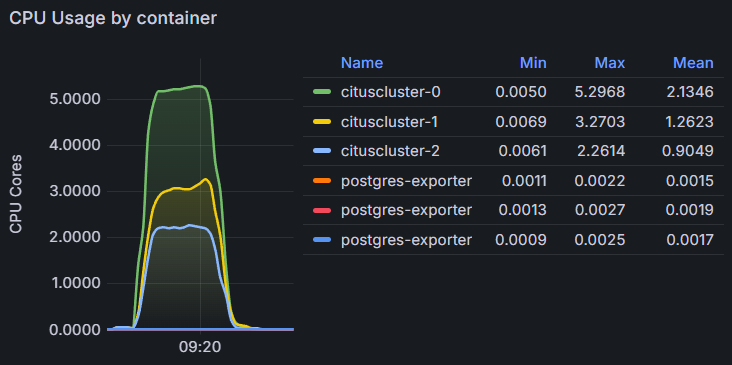
\includegraphics[width=0.8\textwidth]{resources/chapter-4/citusdata-usage.png}
    \caption{Penggunaan CPU CitusData (f2t3)}
    \label{fig:citusdata-usage}
\end{figure}

\textit{Node} cituscluster-0 merupakan koordinator dengan sisanya adalah \textit{worker}. Pada kasus ini, beban pada koordinator cukup tinggi hingga dua kali beban pada satu instans \textit{worker}. Berdasarkan hal tersebut, diketahui bahwa \textit{overhead} pada koordinator memiliki dampak yang signifikan pada kinerja CitusData.

Setelah ditelusuri, terdapat sebuah diskusi pada repositori CitusData yang membahas kinerja CitusData yang buruk pada \textit{benchmark} TPC-C. Terdapat sebuah komentar yang menjawab mengapa hal ini memang wajar. Selain karena CitusData membutuhkan beberapa \textit{network round-trip}, beban TPC-C lebih banyak pada \textit{query planning} dibandingkan dengan eksekusinya \parencite{Slot2020}.

Beban TPC-C dan beban penjualan tiket memiliki kemiripan, sehingga hal yang sama juga berlaku pada kasus ini. Pada penjualan tiket, beban basis data terdiri atas banyak kueri baca dan kueri tulis yang sebenarnya cukup ringan, sehingga koordinator mengalami beban yang tinggi karena harus melakukan tambahan \textit{query planning} untuk koordinasi.

Terdapat alternatif \textit{benchmark} TPC-C yang juga dibahas pada komentar tersebut, yaitu \textit{benchmark} HammerDB. HammerDB menyimpan logika pengujian pada \textit{stored procedure} PostgreSQL. Secara teori, Citus dapat mendelegasikan pemanggilan prosedur tersebut dengan \textit{overhead} yang jauh lebih kecil dan dengan jumlah \textit{network round-trip} yang lebih sedikit \parencite{Slot2020}. Hal ini dibahas lebih lanjut pada artikel yang membahas penggunaan \textit{distributed function} untuk latensi yang lebih baik pada CitusData versi 9 \parencite{Slot2020faster}.

Pendekatan dengan \textit{stored procedure} merupakan alternatif yang dapat dipelajari lebih lanjut pada pengujian lain untuk pengoptimalan yang lebih optimal. Meskipun begitu, permasalahan dari pendekatan ini adalah pemindahan logika bisnis dari kode aplikasi ke basis data. Selain karena keterbatasan sintaks dan dukungan, logika bisnis yang dijalankan pada level aplikasi belum tentu dapat diterjemahkan secara persis menjadi \textit{stored procedure} PostgreSQL.

\subsubsection{Mengapa YugabyteDB tidak perform}

limit koneksi, butuh sumberdaya yang lebih besar. tidak cocok untuk high concurrent transaction. banyak terjadi kegagalan transaksi jadinya diretry.

ambil hasil referensi pengujian juga (pokoknya artikel yg bandingin raw performance)

\subsection{Pengoptimalan Kueri Baca}

buktikan kalau kueri ini banyak banget dipanggil -> pakai grafik/ data dari grafana.

refer ke redis. pakai data pengujian fc postgres (jgn nofc).

apakah hasilnya oke?

\subsection{Integritas Tiket selama Perebutan Tiket}

Apakah terjadi perbedaan data ketersediaan, dropper availability?

Apakah terjadi double booking?

\subsection{Penggunaan Pengendalian Aliran}

Jelasin berapa banyak request yg ditolak (respons 409). Gbs response based on code? atau apa gitu bandingin latensinya fak.

Dampaknya gimana (blm tau).

